\chapter{Cơ sở lý thuyết}
\label{chap:background}

\section{Các khái niệm cơ bản}

Để xây dựng và phân tích hệ thống giao dịch xuyên chuỗi dựa trên intent, cần làm rõ một số khái niệm và mô hình nền tảng trong cả lĩnh vực blockchain và tài chính truyền thống. Các khái niệm này không chỉ giúp hiểu cách các hệ thống hiện tại vận hành mà còn làm rõ những hạn chế, từ đó tạo cơ sở cho hướng tiếp cận được đề xuất trong nghiên cứu này.

Các khái niệm và cơ sở lý thuyết chính bao gồm:

\begin{itemize}
    \item \textbf{Cross-chain bridge}: là cơ chế cho phép chuyển tài sản hoặc dữ liệu giữa các blockchain khác nhau. Các bridge phổ biến thường hoạt động theo mô hình \textit{lock-and-mint} (khóa tài sản trên chain nguồn và phát hành tài sản đại diện trên chain đích) hoặc dựa trên liquidity pool. Mặc dù cho phép hiện thực hóa giao dịch cross-chain, các mô hình này đòi hỏi sự tin cậy vào smart contract, các bên trung gian như relayer hoặc validator, từ đó làm gia tăng rủi ro bảo mật.
    \item \textbf{Cross-chain interaction}: là khái niệm tổng quát bao hàm tất cả các hình thức tương tác giữa các blockchain, bao gồm chuyển tài sản, message và đồng bộ trạng thái. Đây là bài toán phức tạp do sự khác biệt về kiến trúc và cơ chế đồng thuận giữa các chain, đồng thời là nền tảng cho các ứng dụng đa chuỗi hiện đại.
    \item \textbf{Intent-based execution}: là mô hình trong đó người dùng chỉ cần mô tả mục tiêu mong muốn thay vì các bước thực hiện cụ thể. Hệ thống sẽ sử dụng các tác nhân trung gian (solver) để tìm và thực thi phương án tối ưu. Một ví dụ tiêu biểu là CoW Protocol, nơi các lệnh giao dịch được gom lại và xử lý thông qua cơ chế batch auction nhằm tận dụng sự trùng khớp giữa các nhu cầu giao dịch.
    \item \textbf{Atomic swap và HTLC (Hashed Timelock Contract)}: là cơ chế cho phép hai bên trao đổi tài sản giữa các blockchain mà không cần tin cậy lẫn nhau. HTLC sử dụng kết hợp hashlock và timelock để đảm bảo rằng giao dịch chỉ được thực hiện khi cả hai bên đều hoàn thành nghĩa vụ. Tuy nhiên, mô hình này gặp hạn chế về khả năng mở rộng và khó áp dụng trong các hệ thống nhiều bên.
    \item \textbf{Mô hình tài chính truyền thống (SWIFT, Wise)}:
    \begin{itemize}
        \item SWIFT là hệ thống truyền thông giữa các ngân hàng, hỗ trợ chuyển tiền quốc tế nhưng phụ thuộc vào nhiều trung gian, dẫn đến chi phí cao và độ trễ lớn.
        \item Wise (formerly TransferWise) áp dụng cơ chế \textit{netting nội bộ}, cho phép đối soát các dòng tiền đối ứng và giảm thiểu việc chuyển tiền xuyên biên giới thực tế.
    \end{itemize}
\end{itemize}

\section{Các pattern phân loại bridge}

\subsection{Phân loại theo messaging protocol}

Các bridge có thể được phân loại dựa trên cách mà chain đích xác minh trạng thái hoặc giao dịch từ chain nguồn:

\begin{itemize}
    \item \textbf{State validating protocols}: là mô hình trong đó chain đích có thể xác minh trực tiếp trạng thái của chain nguồn dựa trên các giả định bảo mật của blockchain gốc. Mô hình này thường xuất hiện trong các bridge giữa Layer 1 và Layer 2, nơi Layer 1 đóng vai trò là ``source of truth''. Nhờ đó, mức độ bảo mật cao vì không cần tin tưởng bên thứ ba, nhưng chi phí tính toán và triển khai thường lớn.
    \item \textbf{Consensus verifying protocols}: trong mô hình này, chain đích xác minh rằng một giao dịch trên chain nguồn đã được hoàn tất thông qua việc kiểm chứng cơ chế đồng thuận. Điều này thường yêu cầu các bằng chứng (proof) về block hoặc transaction, giúp đảm bảo tính đúng đắn mà không cần tin cậy hoàn toàn vào bên trung gian.
    \item \textbf{Third-party attestation protocols}: là mô hình phổ biến nhất trong thực tế, trong đó một thực thể trung gian (có thể là một validator, một tập hợp multi-signature hoặc một blockchain riêng) xác nhận tính hợp lệ của giao dịch. Ưu điểm là dễ triển khai và hiệu năng cao, nhưng nhược điểm lớn là phụ thuộc vào trust assumption, dẫn đến nhiều rủi ro bảo mật.
    \item \textbf{Optimistic protocols}: dựa trên giả định rằng các giao dịch là hợp lệ trừ khi bị chứng minh ngược lại. Một hoặc nhiều ``watcher'' có thể phát hiện và báo cáo gian lận trong một khoảng thời gian gọi là fraud window. Mô hình này giảm chi phí xác minh ban đầu nhưng yêu cầu cơ chế challenge hiệu quả để đảm bảo an toàn.
\end{itemize}

\subsection{Phân loại theo type of operation}

Bên cạnh messaging protocol, bridge còn được phân loại theo cách thức xử lý tài sản và giao dịch giữa các chain:

\begin{itemize}
    \item \textbf{Liquidity networks}: sử dụng các pool thanh khoản trên nhiều chain. Người dùng gửi tài sản vào pool trên chain nguồn và nhận tài sản tương ứng từ pool trên chain đích. Mô hình này không yêu cầu mint tài sản mới mà tận dụng thanh khoản có sẵn, giúp giảm độ trễ và cải thiện trải nghiệm người dùng, nhưng phụ thuộc vào thanh khoản và có thể gặp rủi ro mất cân bằng pool.
    \item \textbf{Token bridges}: hoạt động theo mô hình khóa (lock) hoặc đốt (burn) tài sản trên chain nguồn và phát hành (mint) tài sản tương ứng trên chain đích. Các token được tạo ra trên chain đích thường là tài sản tổng hợp (wrapped asset), đại diện cho quyền sở hữu tài sản gốc. Đây là mô hình phổ biến nhất nhưng cũng là mục tiêu của nhiều cuộc tấn công do tồn tại các thành phần như custodian và debt issuer.
    \item \textbf{Coordination protocols}: không chỉ tập trung vào chuyển tài sản mà còn hỗ trợ tương tác phức tạp giữa các chain, như gọi hàm, truyền dữ liệu hoặc đồng bộ trạng thái. Mô hình này cho phép xây dựng các ứng dụng đa chuỗi (cross-chain dApps), nhưng đồng thời làm tăng đáng kể độ phức tạp của hệ thống.
\end{itemize}

Từ các khái niệm trên, có thể nhận thấy rằng các hệ thống hiện tại, dù trong blockchain hay tài chính truyền thống, đều phải đối mặt với bài toán tối ưu hóa giữa chi phí, hiệu năng và độ an toàn. Đặc biệt, cơ chế netting trong tài chính truyền thống và mô hình intent-based trong blockchain gợi mở khả năng kết hợp để xây dựng một hệ thống cross-chain hiệu quả hơn, trong đó việc ghép nối các nhu cầu giao dịch có thể thay thế cho việc di chuyển tài sản trực tiếp giữa các chain.

\section{Khảo sát các giải pháp hiện có}

\subsection{Phân loại trực quan}

Để đánh giá tổng quan các kiến trúc bridge hiện nay, tiến hành phân loại các bridge dựa trên các pattern bridge đã trình bày ở mục 2.2: (i) cơ chế truyền thông giữa các chain (communication protocol) và (ii) loại hình vận hành (bridge type). Kết quả được biểu diễn dưới dạng một bảng, trong đó các cột tương ứng với các messaging protocol (state validating, consensus verifying, third-party attestation, optimistic), còn các hàng tương ứng với các loại bridge (liquidity network, token bridge, coordination protocol).

\begin{figure}[H]
  \begin{center}
  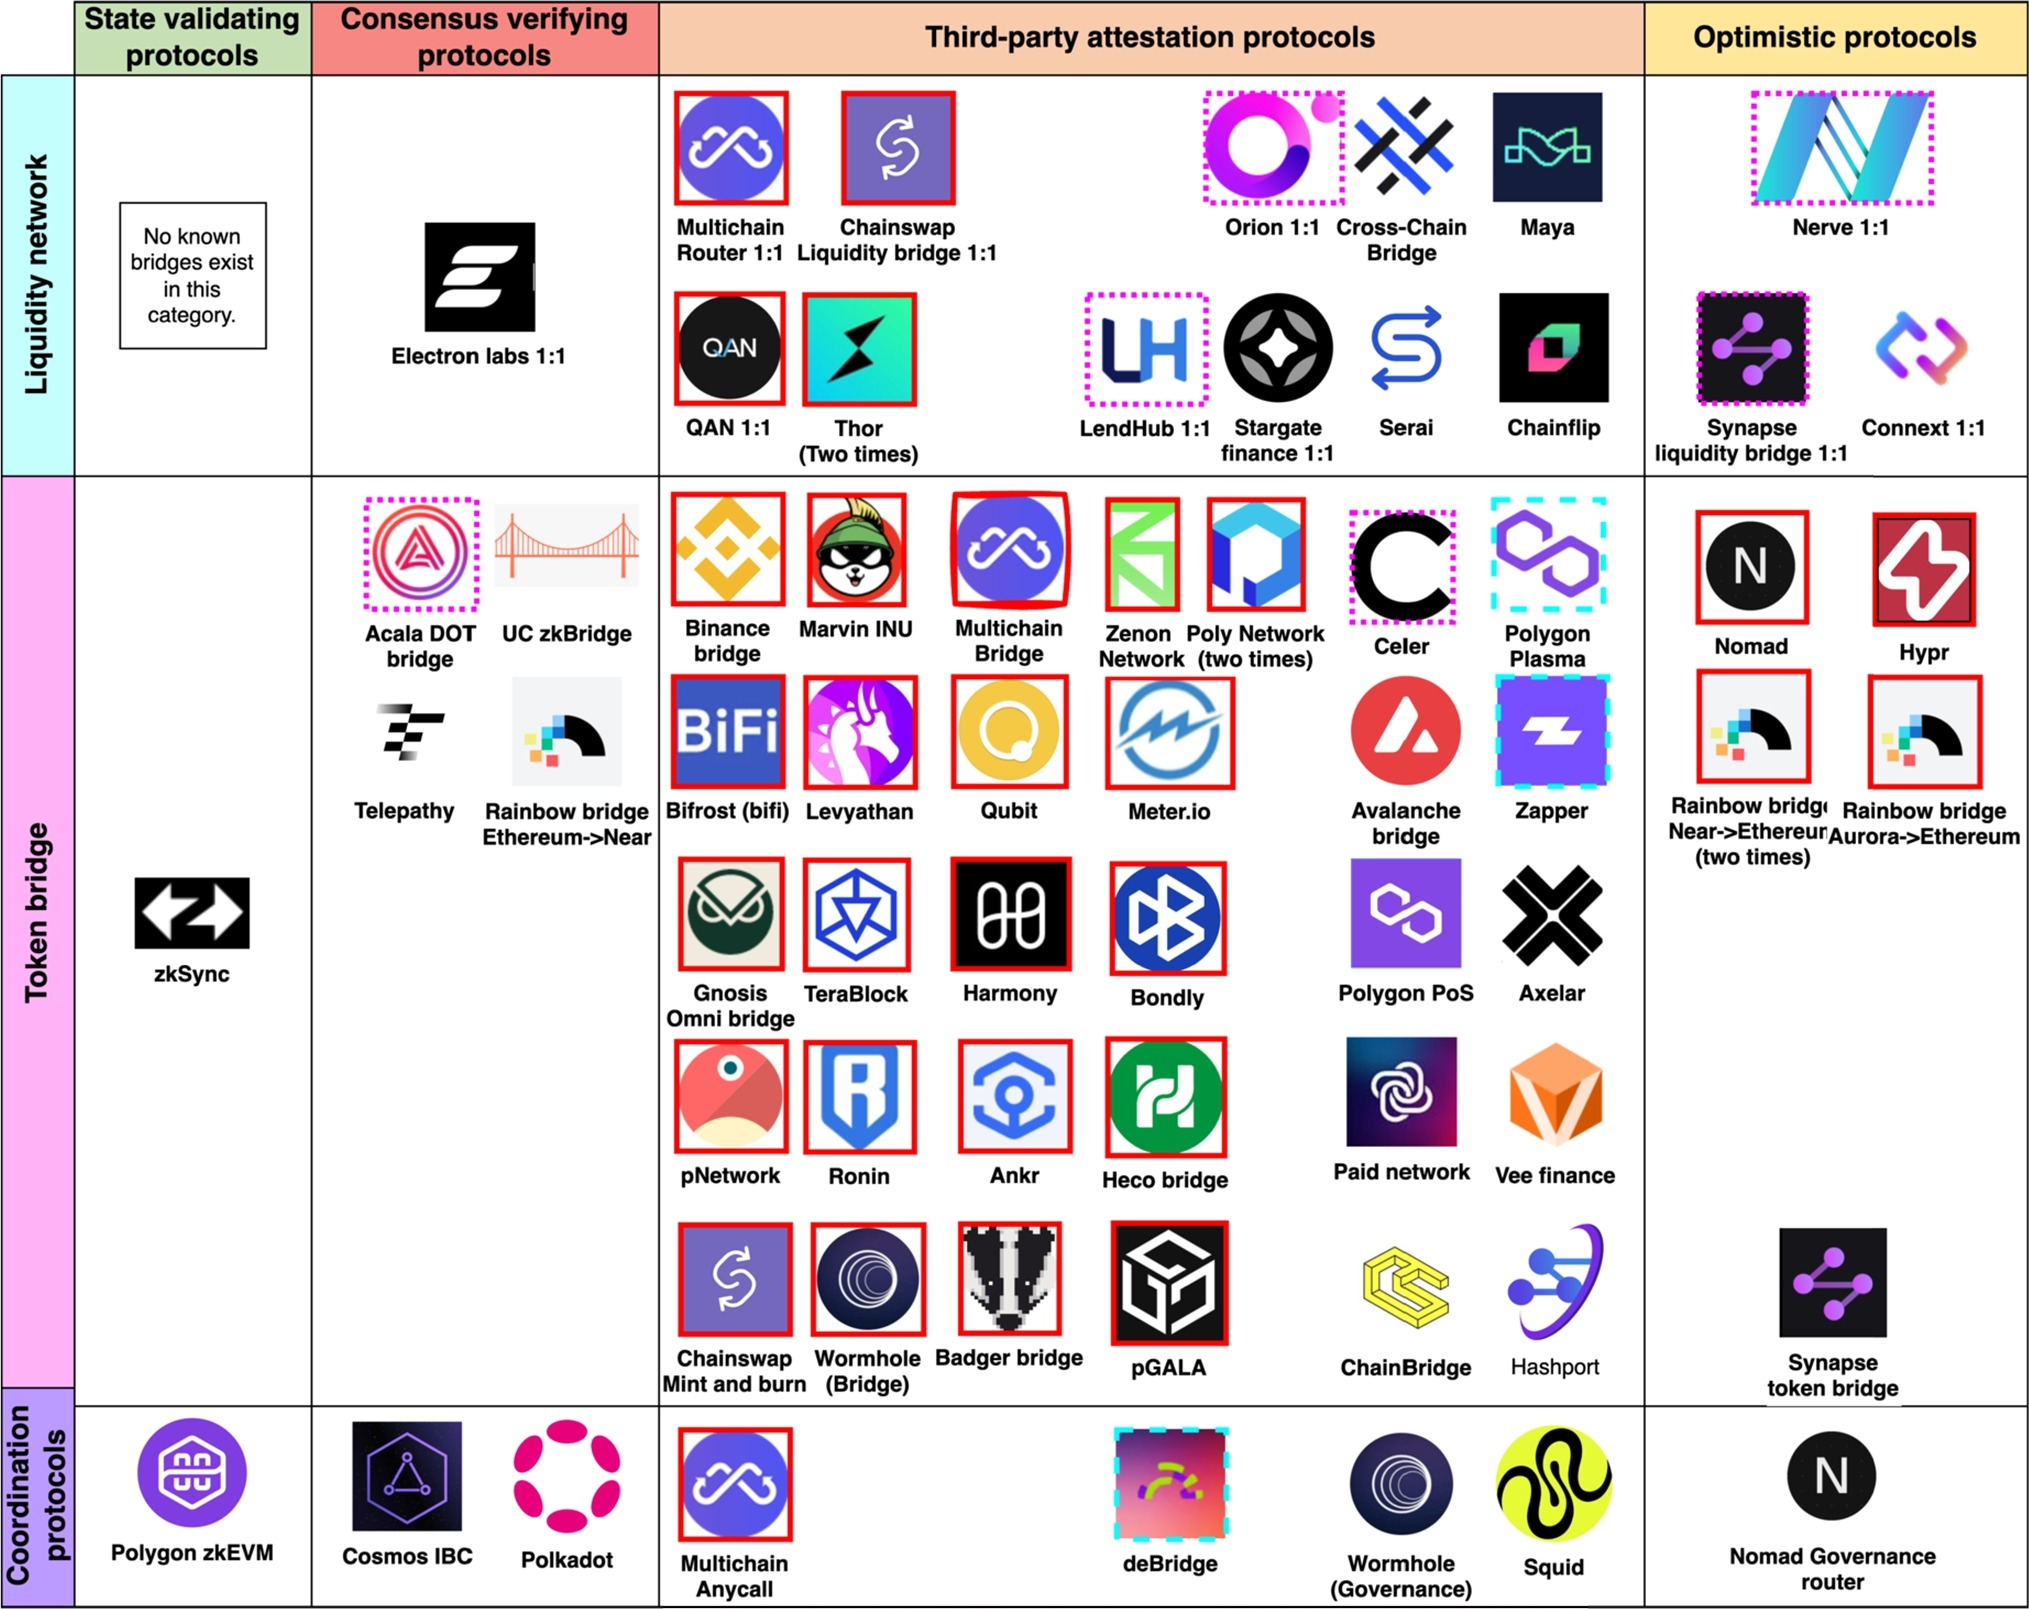
\includegraphics[width=\linewidth]{figures/c1/bridge-taxonomy}
  \end{center}
  \caption{Phân loại các bridge theo messaging protocol và type of operation, đánh dấu trạng thái bảo mật}
  \label{fig:bridge-taxonomy}
\end{figure}

Trong biểu đồ này, mỗi bridge được đánh dấu theo trạng thái bảo mật: các bridge bị tấn công được viền đỏ, các bridge có lỗ hổng đã được phát hiện nhưng chưa bị khai thác được viền xanh lam nét đứt, và các trường hợp nằm ngoài phạm vi nghiên cứu được đánh dấu bằng viền hồng. Cách biểu diễn này cho phép quan sát trực quan mối quan hệ giữa kiến trúc bridge và mức độ rủi ro bảo mật.

\subsection{Đánh giá ưu/nhược của từng nhóm}

Từ kết quả phân loại, có thể rút ra một số nhận định quan trọng về các mô hình bridge hiện tại. Trước hết, phần lớn các bridge trong thực tế được xây dựng dựa trên \textbf{third-party attestation protocols}. Đây là mô hình mà một hoặc một nhóm validator hoặc relayer trung gian xác nhận các giao dịch cross-chain. Các bridge tiêu biểu sử dụng mô hình này bao gồm Binance Bridge, Wormhole, Multichain hay Ronin Network. Ưu điểm của cách tiếp cận này là dễ triển khai và có hiệu năng cao, tuy nhiên nó phụ thuộc mạnh vào giả định tin cậy đối với các thực thể trung gian. Thực tế cho thấy đây cũng chính là điểm yếu bảo mật lớn nhất. Nhiều vụ tấn công nghiêm trọng đã xảy ra trên các bridge thuộc nhóm này, tiêu biểu như Ronin Bridge hack với thiệt hại khoảng 625 triệu USD do attacker kiểm soát majority validator, hay Wormhole hack với khoảng 320 triệu USD do lỗi xác minh chữ ký. Ngoài ra, Binance Bridge cũng từng bị khai thác với thiệt hại hàng trăm triệu USD do forged proof. Các ví dụ này cho thấy rằng khi trust assumption bị phá vỡ, toàn bộ hệ thống bridge có thể bị khai thác trực tiếp. Do đó, có thể kết luận rằng \textbf{third-party attestation là mô hình phổ biến nhất nhưng cũng là yếu nhất về mặt bảo mật}.

Tương tự, các \textbf{optimistic protocols} cũng tồn tại những rủi ro đáng kể. Một số bridge như Nomad hay Rainbow Bridge áp dụng mô hình này, trong đó giao dịch được coi là hợp lệ mặc định và chỉ bị hủy nếu có fraud proof. Tuy nhiên, trong vụ tấn công Nomad năm 2022, một lỗi khởi tạo đã khiến bất kỳ giao dịch nào cũng được coi là hợp lệ, dẫn đến việc hàng trăm triệu USD bị rút khỏi hệ thống. Điều này cho thấy rằng mặc dù optimistic bridge giảm chi phí xác minh ban đầu, nó phụ thuộc mạnh vào cơ chế challenge và watcher, và khi các cơ chế này thất bại, hệ thống có thể bị khai thác trên diện rộng.

Đối với \textbf{consensus verifying protocols}, đây là một hướng tiếp cận có tiềm năng cao về mặt bảo mật vì chain đích có thể xác minh tính hợp lệ của giao dịch dựa trên bằng chứng từ cơ chế đồng thuận của chain nguồn. Một số ví dụ liên quan đến hướng này có thể kể đến các thiết kế relay chain hoặc light client-based bridge trong hệ sinh thái như Cosmos IBC hoặc các nghiên cứu về zkBridge. Tuy nhiên, số lượng bridge thực tế áp dụng mô hình này vẫn còn hạn chế. Nguyên nhân chủ yếu là do chi phí triển khai cao, yêu cầu xác minh phức tạp (ví dụ: light client verification hoặc zk-proof), và khó tích hợp với các blockchain không tương thích. Do đó, mặc dù có ưu điểm về bảo mật, \textbf{consensus verifying chưa được áp dụng rộng rãi trong thực tế}.

Cuối cùng, \textbf{state validating protocols} được xem là mô hình có mức độ bảo mật cao nhất, khi toàn bộ trạng thái của chain nguồn có thể được xác minh trực tiếp trên chain đích. Các bridge giữa Layer 1 và Layer 2 như Optimism hoặc zkSync bridge là ví dụ điển hình, nơi Layer 1 đóng vai trò là nguồn chân lý duy nhất. Tuy nhiên, mô hình này hầu như không được áp dụng cho các bridge giữa các blockchain độc lập do yêu cầu kỹ thuật rất cao, đặc biệt là việc xác minh state hoặc proof một cách hiệu quả. Điều này khiến cho \textbf{state validating có độ an toàn cao nhưng phạm vi ứng dụng còn hạn chế}.

Xét theo góc độ \textbf{type of operation}, có thể nhận thấy rằng phần lớn các bridge hiện nay hoạt động theo mô hình \textbf{token bridge} và \textbf{coordination protocol}. Các bridge như Wormhole, Multichain hay Binance Bridge chủ yếu sử dụng mô hình token bridge với cơ chế lock-and-mint hoặc burn-and-mint. Đây cũng chính là lý do khiến các thành phần như custodian và debt issuer trở thành mục tiêu chính của các cuộc tấn công.

Ngược lại, các \textbf{liquidity network} như ThorChain hoặc một số thiết kế của Across Protocol có cách tiếp cận khác, dựa trên việc sử dụng pool thanh khoản thay vì mint token mới. Mặc dù mô hình này có thể giảm một số rủi ro liên quan đến custodian, nó lại phụ thuộc vào thanh khoản và cơ chế cân bằng giữa các pool, đồng thời chưa chiếm tỷ trọng lớn trong các bridge được khảo sát.

\subsection{Đánh giá các sản phẩm tương tự}
\label{sec:related-products}

% TODO: So sánh chi tiết với các giao thức/sản phẩm tương tự:
% - Chainlink CCIP (Cross-Chain Interoperability Protocol)
% - LayerZero
% - Wormhole
% - Across Protocol
% - Hyperlane / Connext / Axelar
% Tiêu chí so sánh đề xuất: kiến trúc messaging, trust assumption, hỗ trợ
% intent-based, hỗ trợ EVM/non-EVM, độ trễ, chi phí, lịch sử bảo mật.

\subsection{Khoảng trống nghiên cứu}

Từ các phân tích trên, có thể thấy rằng các giải pháp bridge hiện tại chủ yếu đánh đổi giữa hiệu năng và bảo mật. Các mô hình phổ biến như third-party attestation đạt được hiệu năng cao nhưng lại dễ bị khai thác, trong khi các mô hình an toàn hơn như consensus verifying hoặc state validating lại khó triển khai và chưa phổ biến. Điều này cho thấy một khoảng trống rõ ràng trong thiết kế hệ thống cross-chain, nơi cần một cách tiếp cận mới có thể giảm phụ thuộc vào trung gian mà vẫn đảm bảo hiệu quả và an toàn.

\section{Công cụ và nền tảng}

Hệ thống được xây dựng trên một stack công nghệ TypeScript/Node.js hiện đại, với các thành phần chính như sau:

\subsection{Ngôn ngữ và môi trường thực thi}

\begin{itemize}
    \item \textbf{TypeScript}: ngôn ngữ chính của toàn bộ codebase. TypeScript bổ sung hệ thống kiểu tĩnh trên nền JavaScript, giúp phát hiện lỗi sớm tại thời điểm biên dịch và cải thiện khả năng bảo trì cho các module phức tạp như matching engine và liquidity service.
    \item \textbf{Node.js}: môi trường thực thi phía server cho backend, hỗ trợ mô hình bất đồng bộ phù hợp với các tác vụ I/O liên quan đến RPC blockchain và xử lý sự kiện.
    \item \textbf{tsx}: công cụ chạy và watch các tệp TypeScript trực tiếp trong quá trình phát triển, đồng thời được dùng để chạy các bộ kiểm thử (\texttt{tsx --test}).
\end{itemize}

\subsection{Web framework và xác thực dữ liệu}

\begin{itemize}
    \item \textbf{Fastify}: web framework hiệu năng cao cho Node.js, được sử dụng để hiện thực các API HTTP của backend (ví dụ: \texttt{POST /intent}, \texttt{GET /orders/:id}, kênh sự kiện SSE \texttt{GET /orders/:id/events}). Fastify cung cấp routing nhanh, hệ thống plugin mở rộng và tích hợp tốt với TypeScript.
    \item \textbf{@fastify/cors}: plugin chính thức của Fastify để cấu hình CORS, cho phép giao diện người dùng (Next.js frontend) truy cập backend từ origin khác.
    \item \textbf{Zod}: thư viện khai báo và kiểm tra schema cho dữ liệu vào/ra, được dùng để xác thực các trường của intent (ví dụ: \texttt{srcChain}, \texttt{amount}, \texttt{deadline}) trước khi đưa vào tầng xử lý nghiệp vụ.
\end{itemize}

\subsection{Tương tác với blockchain}

\begin{itemize}
    \item \textbf{ethers.js}: thư viện JavaScript phổ biến để tương tác với các blockchain tương thích EVM, hỗ trợ ký giao dịch, gọi smart contract, theo dõi sự kiện và quản lý ví. Trong hệ thống, ethers được sử dụng cho các thao tác cần ABI encoding/decoding và quản lý wallet.
    \item \textbf{viem}: thư viện thế hệ mới cho Ethereum, ưu tiên type-safety và hiệu năng. Viem được dùng song song với ethers để tận dụng API hiện đại và type inference chặt chẽ trong các luồng quan trọng như đọc trạng thái on-chain và mô phỏng giao dịch.
    \item \textbf{dotenv}: nạp biến môi trường (RPC URL, private key của signer kiểm thử, các tham số mạng) từ tệp \texttt{.env}, tách bạch cấu hình môi trường khỏi mã nguồn.
\end{itemize}

\subsection{Công cụ kiểm thử và chất lượng mã}

\begin{itemize}
    \item \textbf{Node Test Runner (\texttt{node:test} qua \texttt{tsx --test})}: bộ chạy kiểm thử tích hợp sẵn trong Node.js, được sử dụng cho các bộ kiểm thử của thuật toán matching, dịch vụ liquidity và luồng matching tổng thể.
    \item \textbf{ESLint} cùng \texttt{@typescript-eslint}: kiểm tra tĩnh và quy ước mã nguồn, đảm bảo nhất quán phong cách lập trình giữa các module.
    \item \textbf{rimraf}: tiện ích cross-platform để dọn thư mục build, dùng trong script \texttt{clean}.
\end{itemize}
